% Options for packages loaded elsewhere
\PassOptionsToPackage{unicode}{hyperref}
\PassOptionsToPackage{hyphens}{url}
%
\documentclass[
]{article}
\usepackage{amsmath,amssymb}
\usepackage{iftex}
\ifPDFTeX
  \usepackage[T1]{fontenc}
  \usepackage[utf8]{inputenc}
  \usepackage{textcomp} % provide euro and other symbols
\else % if luatex or xetex
  \usepackage{unicode-math} % this also loads fontspec
  \defaultfontfeatures{Scale=MatchLowercase}
  \defaultfontfeatures[\rmfamily]{Ligatures=TeX,Scale=1}
\fi
\usepackage{lmodern}
\ifPDFTeX\else
  % xetex/luatex font selection
\fi
% Use upquote if available, for straight quotes in verbatim environments
\IfFileExists{upquote.sty}{\usepackage{upquote}}{}
\IfFileExists{microtype.sty}{% use microtype if available
  \usepackage[]{microtype}
  \UseMicrotypeSet[protrusion]{basicmath} % disable protrusion for tt fonts
}{}
\makeatletter
\@ifundefined{KOMAClassName}{% if non-KOMA class
  \IfFileExists{parskip.sty}{%
    \usepackage{parskip}
  }{% else
    \setlength{\parindent}{0pt}
    \setlength{\parskip}{6pt plus 2pt minus 1pt}}
}{% if KOMA class
  \KOMAoptions{parskip=half}}
\makeatother
\usepackage{xcolor}
\usepackage[margin=1in]{geometry}
\usepackage{color}
\usepackage{fancyvrb}
\newcommand{\VerbBar}{|}
\newcommand{\VERB}{\Verb[commandchars=\\\{\}]}
\DefineVerbatimEnvironment{Highlighting}{Verbatim}{commandchars=\\\{\}}
% Add ',fontsize=\small' for more characters per line
\usepackage{framed}
\definecolor{shadecolor}{RGB}{248,248,248}
\newenvironment{Shaded}{\begin{snugshade}}{\end{snugshade}}
\newcommand{\AlertTok}[1]{\textcolor[rgb]{0.94,0.16,0.16}{#1}}
\newcommand{\AnnotationTok}[1]{\textcolor[rgb]{0.56,0.35,0.01}{\textbf{\textit{#1}}}}
\newcommand{\AttributeTok}[1]{\textcolor[rgb]{0.13,0.29,0.53}{#1}}
\newcommand{\BaseNTok}[1]{\textcolor[rgb]{0.00,0.00,0.81}{#1}}
\newcommand{\BuiltInTok}[1]{#1}
\newcommand{\CharTok}[1]{\textcolor[rgb]{0.31,0.60,0.02}{#1}}
\newcommand{\CommentTok}[1]{\textcolor[rgb]{0.56,0.35,0.01}{\textit{#1}}}
\newcommand{\CommentVarTok}[1]{\textcolor[rgb]{0.56,0.35,0.01}{\textbf{\textit{#1}}}}
\newcommand{\ConstantTok}[1]{\textcolor[rgb]{0.56,0.35,0.01}{#1}}
\newcommand{\ControlFlowTok}[1]{\textcolor[rgb]{0.13,0.29,0.53}{\textbf{#1}}}
\newcommand{\DataTypeTok}[1]{\textcolor[rgb]{0.13,0.29,0.53}{#1}}
\newcommand{\DecValTok}[1]{\textcolor[rgb]{0.00,0.00,0.81}{#1}}
\newcommand{\DocumentationTok}[1]{\textcolor[rgb]{0.56,0.35,0.01}{\textbf{\textit{#1}}}}
\newcommand{\ErrorTok}[1]{\textcolor[rgb]{0.64,0.00,0.00}{\textbf{#1}}}
\newcommand{\ExtensionTok}[1]{#1}
\newcommand{\FloatTok}[1]{\textcolor[rgb]{0.00,0.00,0.81}{#1}}
\newcommand{\FunctionTok}[1]{\textcolor[rgb]{0.13,0.29,0.53}{\textbf{#1}}}
\newcommand{\ImportTok}[1]{#1}
\newcommand{\InformationTok}[1]{\textcolor[rgb]{0.56,0.35,0.01}{\textbf{\textit{#1}}}}
\newcommand{\KeywordTok}[1]{\textcolor[rgb]{0.13,0.29,0.53}{\textbf{#1}}}
\newcommand{\NormalTok}[1]{#1}
\newcommand{\OperatorTok}[1]{\textcolor[rgb]{0.81,0.36,0.00}{\textbf{#1}}}
\newcommand{\OtherTok}[1]{\textcolor[rgb]{0.56,0.35,0.01}{#1}}
\newcommand{\PreprocessorTok}[1]{\textcolor[rgb]{0.56,0.35,0.01}{\textit{#1}}}
\newcommand{\RegionMarkerTok}[1]{#1}
\newcommand{\SpecialCharTok}[1]{\textcolor[rgb]{0.81,0.36,0.00}{\textbf{#1}}}
\newcommand{\SpecialStringTok}[1]{\textcolor[rgb]{0.31,0.60,0.02}{#1}}
\newcommand{\StringTok}[1]{\textcolor[rgb]{0.31,0.60,0.02}{#1}}
\newcommand{\VariableTok}[1]{\textcolor[rgb]{0.00,0.00,0.00}{#1}}
\newcommand{\VerbatimStringTok}[1]{\textcolor[rgb]{0.31,0.60,0.02}{#1}}
\newcommand{\WarningTok}[1]{\textcolor[rgb]{0.56,0.35,0.01}{\textbf{\textit{#1}}}}
\usepackage{graphicx}
\makeatletter
\def\maxwidth{\ifdim\Gin@nat@width>\linewidth\linewidth\else\Gin@nat@width\fi}
\def\maxheight{\ifdim\Gin@nat@height>\textheight\textheight\else\Gin@nat@height\fi}
\makeatother
% Scale images if necessary, so that they will not overflow the page
% margins by default, and it is still possible to overwrite the defaults
% using explicit options in \includegraphics[width, height, ...]{}
\setkeys{Gin}{width=\maxwidth,height=\maxheight,keepaspectratio}
% Set default figure placement to htbp
\makeatletter
\def\fps@figure{htbp}
\makeatother
\setlength{\emergencystretch}{3em} % prevent overfull lines
\providecommand{\tightlist}{%
  \setlength{\itemsep}{0pt}\setlength{\parskip}{0pt}}
\setcounter{secnumdepth}{-\maxdimen} % remove section numbering
\ifLuaTeX
  \usepackage{selnolig}  % disable illegal ligatures
\fi
\IfFileExists{bookmark.sty}{\usepackage{bookmark}}{\usepackage{hyperref}}
\IfFileExists{xurl.sty}{\usepackage{xurl}}{} % add URL line breaks if available
\urlstyle{same}
\hypersetup{
  pdftitle={R Basics},
  pdfauthor={Hadijat Oke 117818512, Thomas Urdinola 117971262},
  hidelinks,
  pdfcreator={LaTeX via pandoc}}

\title{R Basics}
\author{Hadijat Oke 117818512, Thomas Urdinola 117971262}
\date{}

\begin{document}
\maketitle

{
\setcounter{tocdepth}{2}
\tableofcontents
}
\hypertarget{basic-r-manipulation.}{%
\section{Basic R manipulation.}\label{basic-r-manipulation.}}

\begin{enumerate}
\def\labelenumi{\alph{enumi}.}
\tightlist
\item
  In the code segment below, assign the value 2 to variable x, and the
  value 6 to variable y. Then compute the sum `x+y':
\end{enumerate}

\begin{Shaded}
\begin{Highlighting}[]
\CommentTok{\# x \textless{}{-} }
\CommentTok{\# y \textless{}{-} }
\CommentTok{\# print(\_\_\_\_\_)}
\NormalTok{x }\OtherTok{\textless{}{-}} \DecValTok{2}
\NormalTok{y }\OtherTok{\textless{}{-}} \DecValTok{6}
\FunctionTok{print}\NormalTok{(x}\SpecialCharTok{+}\NormalTok{y)}
\end{Highlighting}
\end{Shaded}

\begin{verbatim}
## [1] 8
\end{verbatim}

\begin{enumerate}
\def\labelenumi{\alph{enumi}.}
\setcounter{enumi}{1}
\tightlist
\item
  Construct a list of all even numbers between 1 and 100, assign this to
  the variable `even'. Construct a list of 100 numbers, starting with 1,
  such that the difference between consecutive numbers is three, assign
  this to the variable `threes'. Construct a list of 100 equally spaced
  numbers between 0 and 2. Assign this to the variable x.
\end{enumerate}

\begin{Shaded}
\begin{Highlighting}[]
\NormalTok{even }\OtherTok{=}\FunctionTok{c}\NormalTok{()}
\NormalTok{j }\OtherTok{\textless{}{-}} \DecValTok{1}
\ControlFlowTok{for}\NormalTok{ (i }\ControlFlowTok{in} \DecValTok{1}\SpecialCharTok{:}\DecValTok{100}\NormalTok{)\{}
    \ControlFlowTok{if}\NormalTok{ (i }\SpecialCharTok{\%\%} \DecValTok{2} \SpecialCharTok{==} \DecValTok{0}\NormalTok{)\{}
\NormalTok{      even[j] }\OtherTok{=}\NormalTok{  i}
\NormalTok{      j }\OtherTok{\textless{}{-}}\NormalTok{ j }\SpecialCharTok{+} \DecValTok{1}
\NormalTok{    \}}
\NormalTok{\}}

\NormalTok{threes }\OtherTok{=} \FunctionTok{seq}\NormalTok{(}\AttributeTok{from=}\DecValTok{1}\NormalTok{,}\AttributeTok{to=}\DecValTok{100}\NormalTok{,}\AttributeTok{by=}\DecValTok{3}\NormalTok{)  }
\NormalTok{x }\OtherTok{=} \FunctionTok{seq}\NormalTok{(}\AttributeTok{from =} \DecValTok{0}\NormalTok{, }\AttributeTok{to =} \DecValTok{2}\NormalTok{, }\AttributeTok{length.out =} \DecValTok{100}\NormalTok{)}
\end{Highlighting}
\end{Shaded}

\begin{enumerate}
\def\labelenumi{\alph{enumi}.}
\setcounter{enumi}{2}
\tightlist
\item
  Define a function that computes the square of the input value, call
  this function square:
\end{enumerate}

\begin{Shaded}
\begin{Highlighting}[]
\NormalTok{square }\OtherTok{=} \ControlFlowTok{function}\NormalTok{(num) \{}
\NormalTok{  num}\SpecialCharTok{*}\NormalTok{num}
\NormalTok{\}}
\end{Highlighting}
\end{Shaded}

\begin{enumerate}
\def\labelenumi{\alph{enumi}.}
\setcounter{enumi}{3}
\tightlist
\item
  Plot trigonometric functions sine and cosine for values of x between 0
  and 10. Also plot the `square' function for input values between 0 and
  2.
\end{enumerate}

\begin{Shaded}
\begin{Highlighting}[]
\NormalTok{t }\OtherTok{=} \FunctionTok{seq}\NormalTok{(}\DecValTok{0}\NormalTok{,}\DecValTok{10}\NormalTok{)}
\NormalTok{x }\OtherTok{=} \FunctionTok{seq}\NormalTok{(}\DecValTok{0}\NormalTok{,}\DecValTok{2}\NormalTok{)}
\NormalTok{y1 }\OtherTok{=} \FunctionTok{sin}\NormalTok{(t)}
\NormalTok{y2 }\OtherTok{=} \FunctionTok{cos}\NormalTok{(t)}


\FunctionTok{plot}\NormalTok{(t,y1,}\AttributeTok{type=}\StringTok{"l"}\NormalTok{,}\AttributeTok{col=}\StringTok{"red"}\NormalTok{,}\AttributeTok{xlab=}\StringTok{"x values"}\NormalTok{, }\AttributeTok{ylab=} \StringTok{"y values"}\NormalTok{)}
\FunctionTok{lines}\NormalTok{(t,y2,}\AttributeTok{col=}\StringTok{"green"}\NormalTok{)}
\FunctionTok{lines}\NormalTok{(x,}\FunctionTok{square}\NormalTok{(x),}\AttributeTok{col=}\StringTok{\textquotesingle{}blue\textquotesingle{}}\NormalTok{,}\AttributeTok{type=}\StringTok{\textquotesingle{}l\textquotesingle{}}\NormalTok{)}
\end{Highlighting}
\end{Shaded}

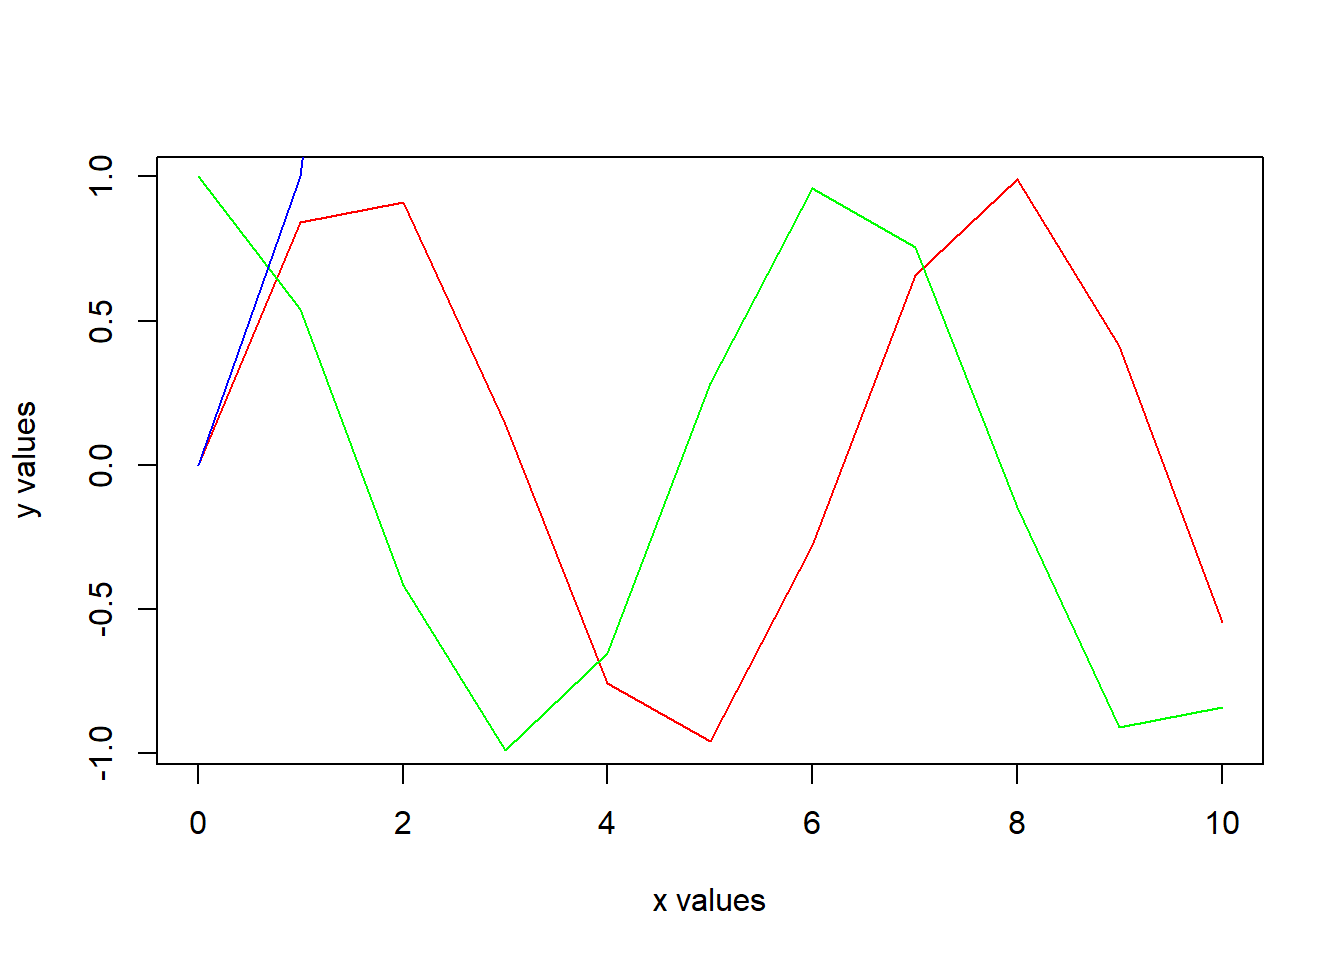
\includegraphics{R_1_files/figure-latex/unnamed-chunk-4-1.pdf}

\hypertarget{working-with-data-in-r.}{%
\section{Working with data in R.}\label{working-with-data-in-r.}}

The dataset `iris' is part of the in-built data repository of R. Use the
`data' command to load the iris dataset.

\begin{Shaded}
\begin{Highlighting}[]
\FunctionTok{data}\NormalTok{(iris)}
\end{Highlighting}
\end{Shaded}

The standard way of storing data in R is a two-dimensional dataframe.
The columns correspond to the the variables and the rows correspond to
observations. To get a sense what the data frame looks like, we use the
`head' command. Apply the head command to the dataframe iris.

\begin{Shaded}
\begin{Highlighting}[]
\FunctionTok{head}\NormalTok{(iris)}
\end{Highlighting}
\end{Shaded}

\begin{verbatim}
##   Sepal.Length Sepal.Width Petal.Length Petal.Width Species
## 1          5.1         3.5          1.4         0.2  setosa
## 2          4.9         3.0          1.4         0.2  setosa
## 3          4.7         3.2          1.3         0.2  setosa
## 4          4.6         3.1          1.5         0.2  setosa
## 5          5.0         3.6          1.4         0.2  setosa
## 6          5.4         3.9          1.7         0.4  setosa
\end{verbatim}

What are the variable/column names in this dataframe?

The column names are: Sepal length, sepal width, petal length, petal
width, and species.

There is an easy way to find all the column names of a dataframe, using
the `colnames' command. Now, apply that command to the iris dataset.

\begin{Shaded}
\begin{Highlighting}[]
\FunctionTok{colnames}\NormalTok{(iris)}
\end{Highlighting}
\end{Shaded}

\begin{verbatim}
## [1] "Sepal.Length" "Sepal.Width"  "Petal.Length" "Petal.Width"  "Species"
\end{verbatim}

We will now work with the data. The first step is to be able to isolate
a column/variable. We do that using the `\$' operator. Assign to x, the
values of the column ``Petal.Length''.

\begin{Shaded}
\begin{Highlighting}[]
\NormalTok{x }\OtherTok{=}\NormalTok{ iris}\SpecialCharTok{$}\NormalTok{Petal.Length}
\end{Highlighting}
\end{Shaded}

Note that x is now a list of numbers, which corresponds to the petal
lenghts of the three different species of the flower iris.

Let us compute the summarry statistics for x, using the min, max, first,
second, and third quartile, and the mean.

\begin{Shaded}
\begin{Highlighting}[]
\FunctionTok{min}\NormalTok{(x)}
\end{Highlighting}
\end{Shaded}

\begin{verbatim}
## [1] 1
\end{verbatim}

\begin{Shaded}
\begin{Highlighting}[]
\FunctionTok{max}\NormalTok{(x)}
\end{Highlighting}
\end{Shaded}

\begin{verbatim}
## [1] 6.9
\end{verbatim}

\begin{Shaded}
\begin{Highlighting}[]
\FunctionTok{quantile}\NormalTok{(x,}\FloatTok{0.25}\NormalTok{)}
\end{Highlighting}
\end{Shaded}

\begin{verbatim}
## 25% 
## 1.6
\end{verbatim}

\begin{Shaded}
\begin{Highlighting}[]
\FunctionTok{quantile}\NormalTok{(x,}\FloatTok{0.50}\NormalTok{)}
\end{Highlighting}
\end{Shaded}

\begin{verbatim}
##  50% 
## 4.35
\end{verbatim}

\begin{Shaded}
\begin{Highlighting}[]
\FunctionTok{quantile}\NormalTok{(x,}\FloatTok{0.75}\NormalTok{)}
\end{Highlighting}
\end{Shaded}

\begin{verbatim}
## 75% 
## 5.1
\end{verbatim}

\begin{Shaded}
\begin{Highlighting}[]
\FunctionTok{mean}\NormalTok{(x)}
\end{Highlighting}
\end{Shaded}

\begin{verbatim}
## [1] 3.758
\end{verbatim}

There is an easy way to summarise these for the entire dataframe using
the summary command. Use this command and compare the values that your
manually computed above to the output of the `summary' command.

\begin{Shaded}
\begin{Highlighting}[]
\FunctionTok{summary}\NormalTok{(iris}\SpecialCharTok{$}\NormalTok{Petal.Length)}
\end{Highlighting}
\end{Shaded}

\begin{verbatim}
##    Min. 1st Qu.  Median    Mean 3rd Qu.    Max. 
##   1.000   1.600   4.350   3.758   5.100   6.900
\end{verbatim}

We want to see if there is any relationship between the variables. To do
so, it is important that we separate data based on the species. Use the
filter command (from the library `dplyr') to create three new dataframes
callled ``setosa'', ``versicolor'', and ``virginica''. Use the ``head''
command to view the first five rows of these data frames.

\begin{Shaded}
\begin{Highlighting}[]
\NormalTok{  setosa }\OtherTok{=} \FunctionTok{head}\NormalTok{(dplyr}\SpecialCharTok{::}\FunctionTok{filter}\NormalTok{(iris, Species }\SpecialCharTok{==} \StringTok{\textquotesingle{}setosa\textquotesingle{}}\NormalTok{))}
\NormalTok{  versicolor }\OtherTok{=} \FunctionTok{head}\NormalTok{(dplyr}\SpecialCharTok{::}\FunctionTok{filter}\NormalTok{(iris, Species }\SpecialCharTok{==} \StringTok{\textquotesingle{}versicolor\textquotesingle{}}\NormalTok{))}
\NormalTok{  virginica }\OtherTok{=} \FunctionTok{head}\NormalTok{(dplyr}\SpecialCharTok{::}\FunctionTok{filter}\NormalTok{(iris, Species }\SpecialCharTok{==} \StringTok{\textquotesingle{}virginica\textquotesingle{}}\NormalTok{))}
\end{Highlighting}
\end{Shaded}

\hypertarget{boxplots-for-iris-data}{%
\section{Boxplots for Iris Data}\label{boxplots-for-iris-data}}

Use the boxplot function to show side-by-side boxplots for the variable
``Petal.Lenght'' across the three different species.

\begin{Shaded}
\begin{Highlighting}[]
\FunctionTok{boxplot}\NormalTok{(setosa}\SpecialCharTok{$}\NormalTok{Petal.Length, versicolor}\SpecialCharTok{$}\NormalTok{Petal.Length, virginica}\SpecialCharTok{$}\NormalTok{Petal.Length, }\AttributeTok{names=}\FunctionTok{c}\NormalTok{(}\StringTok{"setosa"}\NormalTok{, }\StringTok{"versicolor"}\NormalTok{, }\StringTok{"virginica"}\NormalTok{), }\AttributeTok{xlab =} \StringTok{"Species"}\NormalTok{, }\AttributeTok{ylab =} \StringTok{"Petal Length"}\NormalTok{)}
\end{Highlighting}
\end{Shaded}

\includegraphics{R_1_files/figure-latex/unnamed-chunk-12-1.pdf}

Use the boxplot function to show side-by-side boxplots for the variable
``Sepal.Width'' across the three different species.

\begin{Shaded}
\begin{Highlighting}[]
\FunctionTok{boxplot}\NormalTok{(setosa}\SpecialCharTok{$}\NormalTok{Sepal.Width, versicolor}\SpecialCharTok{$}\NormalTok{Sepal.Width, virginica}\SpecialCharTok{$}\NormalTok{Sepal.Width, }\AttributeTok{names=}\FunctionTok{c}\NormalTok{(}\StringTok{"setosa"}\NormalTok{, }\StringTok{"versicolor"}\NormalTok{, }\StringTok{"virginica"}\NormalTok{), }\AttributeTok{xlab =} \StringTok{"Species"}\NormalTok{, }\AttributeTok{ylab =} \StringTok{"Sepal Width"}\NormalTok{)}
\end{Highlighting}
\end{Shaded}

\includegraphics{R_1_files/figure-latex/unnamed-chunk-13-1.pdf}

Note at least two observations that you can make looking at these
boxplots.

There is more variance in speal width than in petal length. Also there
seems to be a correlation between species having a small speal width but
a bigger petal length and vice versa.

\hypertarget{data-visualization-histograms}{%
\section{Data Visualization:
Histograms}\label{data-visualization-histograms}}

Consider the following sample data:

\begin{Shaded}
\begin{Highlighting}[]
\NormalTok{samp\_data }\OtherTok{\textless{}{-}} \FunctionTok{c}\NormalTok{(}\FloatTok{1.54}\NormalTok{,}\FloatTok{0.56}\NormalTok{,}\FloatTok{1.67}\NormalTok{,}\FloatTok{1.54}\NormalTok{,}\FloatTok{1.30}\NormalTok{,}\FloatTok{1.15}\NormalTok{,}\FloatTok{1.59}\NormalTok{,}\SpecialCharTok{{-}}\FloatTok{0.22}\NormalTok{,}\FloatTok{1.01}\NormalTok{,}\FloatTok{1.03}\NormalTok{,}\FloatTok{1.02}\NormalTok{,}\FloatTok{1.77}\NormalTok{,}\FloatTok{1.13}\NormalTok{,}\FloatTok{0.15}\NormalTok{,}\FloatTok{1.02}\NormalTok{,}
               \FloatTok{0.27}\NormalTok{,}\FloatTok{1.40}\NormalTok{,}\FloatTok{0.98}\NormalTok{,}\FloatTok{1.12}\NormalTok{,}\FloatTok{1.12}\NormalTok{,}\FloatTok{0.83}\NormalTok{,}\FloatTok{0.79}\NormalTok{,}\FloatTok{1.29}\NormalTok{,}\FloatTok{0.35}\NormalTok{,}\FloatTok{1.24}\NormalTok{,}\FloatTok{1.35}\NormalTok{,}\FloatTok{0.82}\NormalTok{,}\FloatTok{1.63}\NormalTok{,}\FloatTok{1.34}\NormalTok{,}\FloatTok{0.96}\NormalTok{,}
               \FloatTok{1.37}\NormalTok{,}\FloatTok{0.14}\NormalTok{,}\FloatTok{1.43}\NormalTok{,}\FloatTok{2.00}\NormalTok{,}\FloatTok{1.13}\NormalTok{,}\FloatTok{1.39}\NormalTok{,}\FloatTok{1.18}\NormalTok{,}\FloatTok{0.99}\NormalTok{,}\FloatTok{0.65}\NormalTok{,}\FloatTok{0.88}\NormalTok{,}\FloatTok{1.11}\NormalTok{,}\FloatTok{1.63}\NormalTok{,}\FloatTok{1.53}\NormalTok{,}\FloatTok{0.91}\NormalTok{,}\FloatTok{0.02}\NormalTok{,}
               \FloatTok{0.84}\NormalTok{,}\FloatTok{1.54}\NormalTok{,}\FloatTok{1.21}\NormalTok{,}\FloatTok{1.56}\NormalTok{,}\FloatTok{1.02}\NormalTok{,}\FloatTok{0.87}\NormalTok{,}\FloatTok{0.63}\NormalTok{,}\FloatTok{1.68}\NormalTok{,}\FloatTok{0.71}\NormalTok{,}\FloatTok{1.43}\NormalTok{,}\FloatTok{0.42}\NormalTok{,}\FloatTok{0.80}\NormalTok{,}\FloatTok{1.40}\NormalTok{,}\FloatTok{1.45}\NormalTok{,}\FloatTok{1.34}\NormalTok{,}
               \FloatTok{1.57}\NormalTok{,}\FloatTok{0.98}\NormalTok{,}\FloatTok{0.99}\NormalTok{,}\FloatTok{1.04}\NormalTok{,}\FloatTok{1.15}\NormalTok{,}\FloatTok{0.47}\NormalTok{,}\FloatTok{0.82}\NormalTok{,}\FloatTok{0.89}\NormalTok{,}\FloatTok{0.78}\NormalTok{,}\FloatTok{1.02}\NormalTok{,}\FloatTok{1.56}\NormalTok{,}\FloatTok{1.67}\NormalTok{,}\FloatTok{1.32}\NormalTok{,}\FloatTok{1.23}\NormalTok{,}\FloatTok{0.46}\NormalTok{,}
               \SpecialCharTok{{-}}\FloatTok{0.06}\NormalTok{,}\FloatTok{0.90}\NormalTok{,}\FloatTok{0.94}\NormalTok{,}\FloatTok{1.60}\NormalTok{,}\FloatTok{0.52}\NormalTok{,}\FloatTok{1.04}\NormalTok{,}\FloatTok{1.79}\NormalTok{,}\FloatTok{0.66}\NormalTok{,}\FloatTok{0.76}\NormalTok{,}\FloatTok{1.47}\NormalTok{,}\FloatTok{0.68}\NormalTok{,}\FloatTok{1.38}\NormalTok{,}\FloatTok{0.35}\NormalTok{,}\FloatTok{1.30}\NormalTok{,}\FloatTok{1.30}\NormalTok{,}
               \FloatTok{0.89}\NormalTok{,}\FloatTok{1.62}\NormalTok{,}\FloatTok{0.66}\NormalTok{,}\FloatTok{0.97}\NormalTok{,}\FloatTok{1.27}\NormalTok{,}\FloatTok{1.03}\NormalTok{,}\FloatTok{1.12}\NormalTok{,}\FloatTok{0.48}\NormalTok{,}\FloatTok{0.97}\NormalTok{,}\FloatTok{0.77}\NormalTok{,}\FloatTok{3.00}\NormalTok{,}\FloatTok{3.30}\NormalTok{,}\FloatTok{2.73}\NormalTok{,}\FloatTok{3.21}\NormalTok{,}\FloatTok{3.92}\NormalTok{,}
               \FloatTok{3.33}\NormalTok{,}\FloatTok{2.25}\NormalTok{,}\FloatTok{2.58}\NormalTok{,}\FloatTok{3.45}\NormalTok{,}\FloatTok{2.86}\NormalTok{,}\FloatTok{3.01}\NormalTok{,}\FloatTok{3.27}\NormalTok{,}\FloatTok{2.65}\NormalTok{,}\FloatTok{3.48}\NormalTok{,}\FloatTok{3.18}\NormalTok{,}\FloatTok{2.01}\NormalTok{,}\FloatTok{3.42}\NormalTok{,}\FloatTok{2.13}\NormalTok{,}\FloatTok{3.15}\NormalTok{,}\FloatTok{2.77}\NormalTok{,}
               \FloatTok{2.98}\NormalTok{,}\FloatTok{3.18}\NormalTok{,}\FloatTok{3.20}\NormalTok{,}\FloatTok{2.96}\NormalTok{,}\FloatTok{2.79}\NormalTok{,}\FloatTok{3.15}\NormalTok{,}\FloatTok{3.42}\NormalTok{,}\FloatTok{2.16}\NormalTok{,}\FloatTok{3.41}\NormalTok{,}\FloatTok{3.31}\NormalTok{,}\FloatTok{3.52}\NormalTok{,}\FloatTok{3.28}\NormalTok{,}\FloatTok{3.90}\NormalTok{,}\FloatTok{3.25}\NormalTok{,}\FloatTok{2.91}\NormalTok{,}
               \FloatTok{2.98}\NormalTok{,}\FloatTok{3.25}\NormalTok{,}\FloatTok{3.02}\NormalTok{,}\FloatTok{2.52}\NormalTok{,}\FloatTok{2.97}\NormalTok{,}\FloatTok{2.31}\NormalTok{,}\FloatTok{3.30}\NormalTok{,}\FloatTok{2.50}\NormalTok{,}\FloatTok{3.19}\NormalTok{,}\FloatTok{2.46}\NormalTok{,}\FloatTok{2.82}\NormalTok{,}\FloatTok{2.83}\NormalTok{,}\FloatTok{2.48}\NormalTok{,}\FloatTok{2.55}\NormalTok{,}\FloatTok{3.18}\NormalTok{,}
               \FloatTok{3.56}\NormalTok{,}\FloatTok{3.69}\NormalTok{,}\FloatTok{3.04}\NormalTok{,}\FloatTok{2.91}\NormalTok{,}\FloatTok{2.94}\NormalTok{,}\FloatTok{2.81}\NormalTok{,}\FloatTok{2.93}\NormalTok{,}\FloatTok{3.11}\NormalTok{,}\FloatTok{2.28}\NormalTok{,}\FloatTok{2.63}\NormalTok{,}\FloatTok{3.37}\NormalTok{,}\FloatTok{3.49}\NormalTok{,}\FloatTok{3.08}\NormalTok{,}\FloatTok{3.49}\NormalTok{,}\FloatTok{2.49}\NormalTok{,}
               \FloatTok{2.89}\NormalTok{,}\FloatTok{3.15}\NormalTok{,}\FloatTok{3.21}\NormalTok{,}\FloatTok{2.79}\NormalTok{,}\FloatTok{3.46}\NormalTok{,}\FloatTok{3.56}\NormalTok{,}\FloatTok{3.33}\NormalTok{,}\FloatTok{3.15}\NormalTok{,}\FloatTok{2.18}\NormalTok{,}\FloatTok{3.08}\NormalTok{,}\FloatTok{2.24}\NormalTok{,}\FloatTok{4.31}\NormalTok{,}\FloatTok{3.23}\NormalTok{,}\FloatTok{3.35}\NormalTok{,}\FloatTok{3.18}\NormalTok{,}
               \FloatTok{3.08}\NormalTok{,}\FloatTok{3.79}\NormalTok{,}\FloatTok{2.44}\NormalTok{,}\FloatTok{3.04}\NormalTok{,}\FloatTok{2.36}\NormalTok{,}\FloatTok{2.23}\NormalTok{,}\FloatTok{3.55}\NormalTok{,}\FloatTok{2.70}\NormalTok{,}\FloatTok{3.01}\NormalTok{,}\FloatTok{3.48}\NormalTok{,}\FloatTok{3.68}\NormalTok{,}\FloatTok{3.37}\NormalTok{,}\FloatTok{3.01}\NormalTok{,}\FloatTok{3.18}\NormalTok{,}\FloatTok{2.13}\NormalTok{,}
               \FloatTok{3.39}\NormalTok{,}\FloatTok{3.37}\NormalTok{,}\FloatTok{2.86}\NormalTok{,}\FloatTok{3.34}\NormalTok{,}\FloatTok{3.16}\NormalTok{,}\FloatTok{2.54}\NormalTok{,}\FloatTok{3.58}\NormalTok{,}\FloatTok{3.63}\NormalTok{,}\FloatTok{2.43}\NormalTok{,}\FloatTok{3.94}\NormalTok{,}\FloatTok{2.80}\NormalTok{,}\FloatTok{2.41}\NormalTok{,}\FloatTok{2.25}\NormalTok{,}\FloatTok{2.87}\NormalTok{,}\FloatTok{3.17}\NormalTok{,}
               \FloatTok{2.07}\NormalTok{,}\FloatTok{2.63}\NormalTok{,}\FloatTok{2.99}\NormalTok{,}\FloatTok{3.21}\NormalTok{,}\FloatTok{2.57}\NormalTok{,}\FloatTok{2.93}\NormalTok{,}\FloatTok{3.32}\NormalTok{,}\FloatTok{2.49}\NormalTok{,}\FloatTok{1.89}\NormalTok{,}\FloatTok{2.98}\NormalTok{,}\FloatTok{2.83}\NormalTok{,}\FloatTok{3.80}\NormalTok{,}\FloatTok{2.92}\NormalTok{,}\FloatTok{2.90}\NormalTok{,}\FloatTok{3.00}\NormalTok{,}
               \FloatTok{3.10}\NormalTok{,}\FloatTok{2.41}\NormalTok{,}\FloatTok{2.66}\NormalTok{,}\FloatTok{2.77}\NormalTok{,}\FloatTok{2.69}\NormalTok{,}\FloatTok{2.99}\NormalTok{,}\FloatTok{2.50}\NormalTok{,}\FloatTok{3.21}\NormalTok{,}\FloatTok{2.98}\NormalTok{,}\FloatTok{3.45}\NormalTok{,}\FloatTok{3.83}\NormalTok{,}\FloatTok{3.00}\NormalTok{,}\FloatTok{2.54}\NormalTok{,}\FloatTok{3.86}\NormalTok{,}\FloatTok{2.80}\NormalTok{,}
               \FloatTok{2.83}\NormalTok{,}\FloatTok{2.97}\NormalTok{,}\FloatTok{2.36}\NormalTok{,}\FloatTok{2.88}\NormalTok{,}\FloatTok{3.05}\NormalTok{,}\FloatTok{2.89}\NormalTok{,}\FloatTok{1.71}\NormalTok{,}\FloatTok{3.64}\NormalTok{,}\FloatTok{2.49}\NormalTok{,}\FloatTok{3.45}\NormalTok{,}\FloatTok{3.41}\NormalTok{,}\FloatTok{3.01}\NormalTok{,}\FloatTok{2.57}\NormalTok{,}\FloatTok{3.87}\NormalTok{,}\FloatTok{3.23}\NormalTok{,}
               \FloatTok{2.57}\NormalTok{,}\FloatTok{2.56}\NormalTok{,}\FloatTok{2.85}\NormalTok{,}\FloatTok{2.83}\NormalTok{,}\FloatTok{3.19}\NormalTok{,}\FloatTok{3.15}\NormalTok{,}\FloatTok{3.17}\NormalTok{,}\FloatTok{2.90}\NormalTok{,}\FloatTok{3.29}\NormalTok{,}\FloatTok{3.46}\NormalTok{,}\FloatTok{2.43}\NormalTok{,}\FloatTok{3.04}\NormalTok{,}\FloatTok{2.81}\NormalTok{,}\FloatTok{3.28}\NormalTok{,}\FloatTok{2.82}\NormalTok{,}
               \FloatTok{3.00}\NormalTok{,}\FloatTok{3.78}\NormalTok{,}\FloatTok{3.16}\NormalTok{,}\FloatTok{3.96}\NormalTok{,}\FloatTok{4.03}\NormalTok{,}\FloatTok{3.57}\NormalTok{,}\FloatTok{3.95}\NormalTok{,}\FloatTok{3.20}\NormalTok{,}\FloatTok{2.41}\NormalTok{,}\FloatTok{2.58}\NormalTok{,}\FloatTok{2.79}\NormalTok{,}\FloatTok{3.23}\NormalTok{,}\FloatTok{2.77}\NormalTok{,}\FloatTok{2.97}\NormalTok{,}\FloatTok{3.34}\NormalTok{,}
               \FloatTok{3.13}\NormalTok{,}\FloatTok{3.78}\NormalTok{,}\FloatTok{2.70}\NormalTok{,}\FloatTok{3.14}\NormalTok{,}\FloatTok{3.25}\NormalTok{,}\FloatTok{2.26}\NormalTok{,}\FloatTok{3.99}\NormalTok{,}\FloatTok{3.10}\NormalTok{,}\FloatTok{3.76}\NormalTok{,}\FloatTok{2.92}\NormalTok{,}\FloatTok{2.69}\NormalTok{,}\FloatTok{3.58}\NormalTok{,}\FloatTok{3.11}\NormalTok{,}\FloatTok{3.59}\NormalTok{,}\FloatTok{2.74}\NormalTok{,}
               \FloatTok{3.82}\NormalTok{,}\FloatTok{2.07}\NormalTok{,}\FloatTok{2.81}\NormalTok{,}\FloatTok{1.74}\NormalTok{,}\FloatTok{3.45}\NormalTok{,}\FloatTok{3.38}\NormalTok{,}\FloatTok{3.74}\NormalTok{,}\FloatTok{2.79}\NormalTok{,}\FloatTok{2.71}\NormalTok{,}\FloatTok{2.83}\NormalTok{,}\FloatTok{2.74}\NormalTok{,}\FloatTok{1.58}\NormalTok{,}\FloatTok{2.94}\NormalTok{,}\FloatTok{3.53}\NormalTok{,}\FloatTok{3.01}\NormalTok{,}
               \FloatTok{2.21}\NormalTok{,}\FloatTok{2.61}\NormalTok{,}\FloatTok{2.95}\NormalTok{,}\FloatTok{2.58}\NormalTok{,}\FloatTok{3.92}\NormalTok{,}\FloatTok{2.68}\NormalTok{,}\FloatTok{2.85}\NormalTok{,}\FloatTok{3.06}\NormalTok{,}\FloatTok{2.86}\NormalTok{,}\FloatTok{3.43}\NormalTok{,}\FloatTok{3.16}\NormalTok{,}\FloatTok{3.02}\NormalTok{,}\FloatTok{2.29}\NormalTok{,}\FloatTok{3.74}\NormalTok{,}\FloatTok{3.49}\NormalTok{,}
               \FloatTok{4.04}\NormalTok{,}\FloatTok{1.66}\NormalTok{,}\FloatTok{2.98}\NormalTok{,}\FloatTok{1.70}\NormalTok{,}\FloatTok{3.80}\NormalTok{,}\FloatTok{3.47}\NormalTok{,}\FloatTok{3.26}\NormalTok{,}\FloatTok{2.55}\NormalTok{,}\FloatTok{2.92}\NormalTok{,}\FloatTok{3.46}\NormalTok{,}\FloatTok{3.28}\NormalTok{,}\FloatTok{3.31}\NormalTok{,}\FloatTok{2.32}\NormalTok{,}\FloatTok{2.78}\NormalTok{,}\FloatTok{4.08}\NormalTok{,}
               \FloatTok{3.78}\NormalTok{,}\FloatTok{2.49}\NormalTok{,}\FloatTok{3.26}\NormalTok{,}\FloatTok{2.88}\NormalTok{,}\FloatTok{3.23}\NormalTok{,}\FloatTok{3.15}\NormalTok{,}\FloatTok{2.62}\NormalTok{,}\FloatTok{3.73}\NormalTok{,}\FloatTok{3.03}\NormalTok{,}\FloatTok{2.78}\NormalTok{,}\FloatTok{3.00}\NormalTok{,}\FloatTok{2.61}\NormalTok{,}\FloatTok{2.48}\NormalTok{,}\FloatTok{2.03}\NormalTok{,}\FloatTok{3.04}\NormalTok{,}
               \FloatTok{3.64}\NormalTok{,}\FloatTok{3.43}\NormalTok{,}\FloatTok{3.27}\NormalTok{,}\FloatTok{2.41}\NormalTok{,}\FloatTok{3.60}\NormalTok{,}\FloatTok{2.75}\NormalTok{,}\FloatTok{2.94}\NormalTok{,}\FloatTok{3.23}\NormalTok{,}\FloatTok{3.22}\NormalTok{,}\FloatTok{2.81}\NormalTok{,}\FloatTok{2.72}\NormalTok{,}\FloatTok{3.62}\NormalTok{,}\FloatTok{2.94}\NormalTok{,}\FloatTok{3.17}\NormalTok{,}\FloatTok{3.11}\NormalTok{,}
               \FloatTok{2.60}\NormalTok{,}\FloatTok{3.11}\NormalTok{,}\FloatTok{3.45}\NormalTok{,}\FloatTok{2.37}\NormalTok{,}\FloatTok{3.07}\NormalTok{,}\FloatTok{3.09}\NormalTok{,}\FloatTok{3.90}\NormalTok{,}\FloatTok{2.86}\NormalTok{,}\FloatTok{3.23}\NormalTok{,}\FloatTok{3.50}\NormalTok{,}\FloatTok{2.84}\NormalTok{,}\FloatTok{2.17}\NormalTok{,}\FloatTok{2.58}\NormalTok{,}\FloatTok{3.57}\NormalTok{,}\FloatTok{2.95}\NormalTok{,}
               \FloatTok{2.56}\NormalTok{,}\FloatTok{2.42}\NormalTok{,}\FloatTok{3.38}\NormalTok{,}\FloatTok{3.28}\NormalTok{,}\FloatTok{3.19}\NormalTok{,}\FloatTok{2.77}\NormalTok{,}\FloatTok{3.27}\NormalTok{,}\FloatTok{4.01}\NormalTok{,}\FloatTok{3.65}\NormalTok{,}\FloatTok{3.39}\NormalTok{)}
\FunctionTok{mean}\NormalTok{(samp\_data)}
\end{Highlighting}
\end{Shaded}

\begin{verbatim}
## [1] 2.53215
\end{verbatim}

Use the `hist' function to visualize samp\_data. Furthermore, use
different values of for the ``breaks'' parameter, which species the
number of bins, to explore the shape of the data.

\begin{Shaded}
\begin{Highlighting}[]
  \FunctionTok{hist}\NormalTok{(samp\_data)}
\end{Highlighting}
\end{Shaded}

\includegraphics{R_1_files/figure-latex/unnamed-chunk-15-1.pdf}

\begin{Shaded}
\begin{Highlighting}[]
  \FunctionTok{hist}\NormalTok{(samp\_data,}\AttributeTok{breaks =} \FloatTok{1.0}\NormalTok{, }\AttributeTok{main =} \StringTok{"With breaks 1.0"}\NormalTok{)}
\end{Highlighting}
\end{Shaded}

\includegraphics{R_1_files/figure-latex/unnamed-chunk-15-2.pdf}

\begin{Shaded}
\begin{Highlighting}[]
  \FunctionTok{hist}\NormalTok{(samp\_data,}\AttributeTok{breaks =} \FloatTok{1.5}\NormalTok{, }\AttributeTok{main =} \StringTok{"With breaks 1.5"}\NormalTok{)}
\end{Highlighting}
\end{Shaded}

\includegraphics{R_1_files/figure-latex/unnamed-chunk-15-3.pdf}

\begin{Shaded}
\begin{Highlighting}[]
  \FunctionTok{hist}\NormalTok{(samp\_data,}\AttributeTok{breaks =} \FloatTok{2.0}\NormalTok{, }\AttributeTok{main =} \StringTok{"With breaks 2.0"}\NormalTok{)}
\end{Highlighting}
\end{Shaded}

\includegraphics{R_1_files/figure-latex/unnamed-chunk-15-4.pdf}

\begin{Shaded}
\begin{Highlighting}[]
  \FunctionTok{hist}\NormalTok{(samp\_data,}\AttributeTok{breaks =} \FloatTok{2.5}\NormalTok{, }\AttributeTok{main =} \StringTok{"With breaks 2.5"}\NormalTok{)}
\end{Highlighting}
\end{Shaded}

\includegraphics{R_1_files/figure-latex/unnamed-chunk-15-5.pdf}

\begin{Shaded}
\begin{Highlighting}[]
  \FunctionTok{hist}\NormalTok{(samp\_data,}\AttributeTok{breaks =} \FloatTok{3.0}\NormalTok{, }\AttributeTok{main =} \StringTok{"With breaks 3.0"}\NormalTok{)}
\end{Highlighting}
\end{Shaded}

\includegraphics{R_1_files/figure-latex/unnamed-chunk-15-6.pdf}

\begin{Shaded}
\begin{Highlighting}[]
  \FunctionTok{hist}\NormalTok{(samp\_data,}\AttributeTok{breaks =} \FloatTok{3.5}\NormalTok{, }\AttributeTok{main =} \StringTok{"With breaks 3.5"}\NormalTok{)}
\end{Highlighting}
\end{Shaded}

\includegraphics{R_1_files/figure-latex/unnamed-chunk-15-7.pdf}

\begin{Shaded}
\begin{Highlighting}[]
  \FunctionTok{hist}\NormalTok{(samp\_data,}\AttributeTok{breaks =} \FloatTok{4.0}\NormalTok{, }\AttributeTok{main =} \StringTok{"With breaks 4.0"}\NormalTok{)}
\end{Highlighting}
\end{Shaded}

\includegraphics{R_1_files/figure-latex/unnamed-chunk-15-8.pdf}

\begin{Shaded}
\begin{Highlighting}[]
  \FunctionTok{hist}\NormalTok{(samp\_data, }\AttributeTok{breaks =} \FloatTok{4.5}\NormalTok{, }\AttributeTok{main =}\StringTok{"With breaks 4.5"}\NormalTok{)}
\end{Highlighting}
\end{Shaded}

\includegraphics{R_1_files/figure-latex/unnamed-chunk-15-9.pdf}

What are some good values for the ``breaks'' parameter? Why?

As we see from the histograms, the higher the breaks parameter is, the
more populated our cells are. This means that we are able to analyze our
data more clearly.

Is the sample mean a good measure of location for this dataset? Why?

The mean of the sample data is 2.53215, according to the mean()
function. As we look at our histograms, we see that every break always
includes the mean in the populated data cells as part of our data set,
meaning that it is a good measure of location.

\end{document}
